%%%%%%%%%%%%%%%%%%%%%%
%\appendix[Appendix A: Example I]{Appendix A: Example I} 
\appendix[Waveform, spectrogram and SNR of frog species from David Stewart's CD]{Waveform, spectrogram and SNR of frog species from David Stewart's CD} 

\begin{table}[htb!]
\centering
\caption[Waveform, spectrogram, and SNR of CD]{Waveform, spectrogram, and SNR of selected six frog species from David Stewart's CD}
\label{tab:wav_spec_cd}
\begin{tabular}{llll}
\hline\hline
\backslashbox{Frog \\ species}{}        & Waveform & Spectrogram & SNR (dB)   \\ \hline
\textit{Bufo marinus}        &   
\begin{minipage}{.3\textwidth} 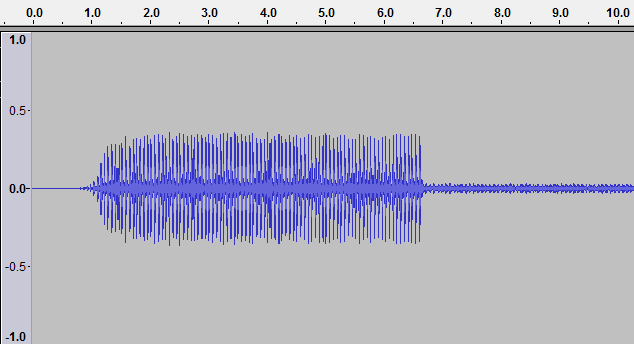
\includegraphics[width=45mm, height=30mm]{image/Ch1/toad_wave.png}  \end{minipage}    &   \begin{minipage}{.3\textwidth} 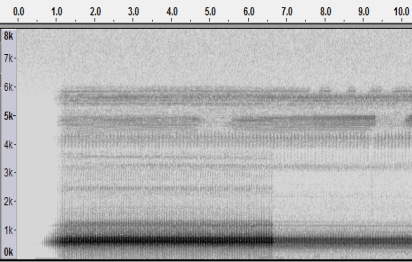
\includegraphics[width=45mm, height=30mm]{image/Ch1/toad_spec.png}  \end{minipage}          & 19.35 \\ \hline
\textit{Litoria caerulea}    &  \begin{minipage}{.3\textwidth} 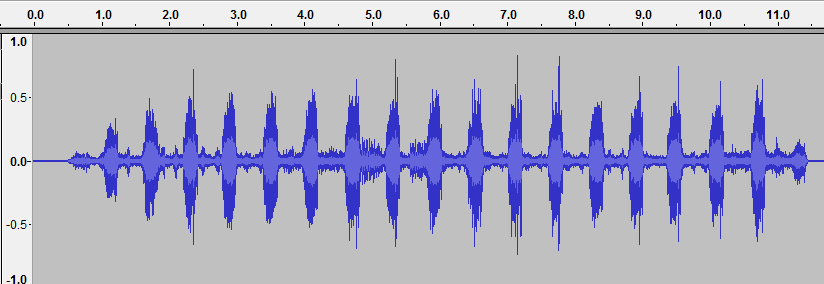
\includegraphics[width=45mm, height=30mm]{image/Ch1/caerulea_wav.png}  \end{minipage}      &     \begin{minipage}{.3\textwidth} 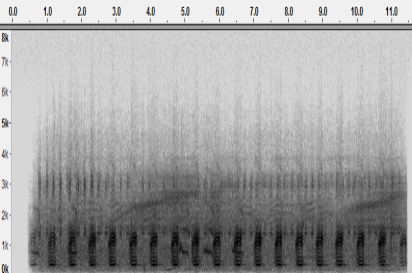
\includegraphics[width=45mm, height=30mm]{image/Ch1/caerulea_spec.png}   \end{minipage}     & 15.78 \\ \hline
\textit{Litoria fallax}      &      \begin{minipage}{.3\textwidth} 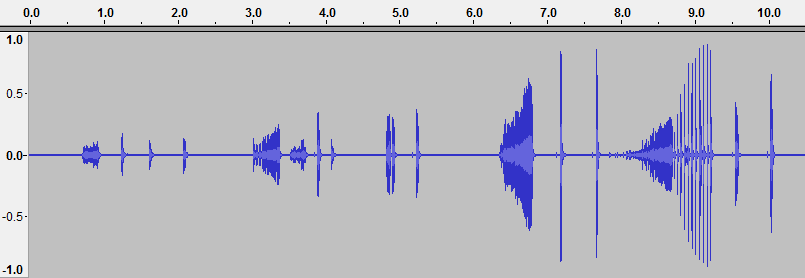
\includegraphics[width=45mm, height=30mm]{image/Ch1/fallax_wav.png} \end{minipage}   &   \begin{minipage}{.3\textwidth} 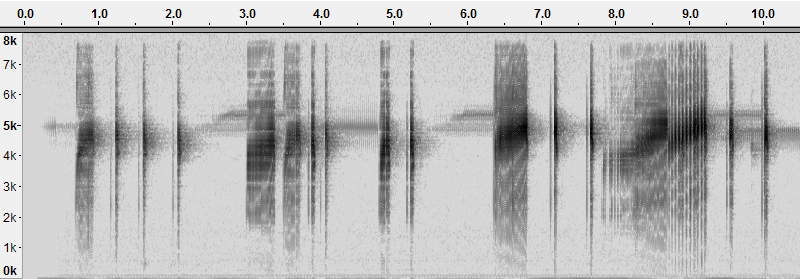
\includegraphics[width=45mm, height=30mm]{image/Ch1/fallax_spec.png}   \end{minipage}       & 43.7  \\ \hline
\end{tabular}
\end{table}




\begin{table}[htb!]
\centering
\begin{tabular}{llll}
\hline
\textit{Litoria gracillenta} &     \begin{minipage}{.3\textwidth} 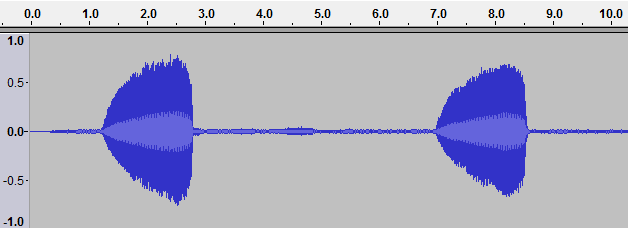
\includegraphics[width=45mm, height=30mm]{image/Ch1/graci_wav.png}  \end{minipage}   &    \begin{minipage}{.3\textwidth} 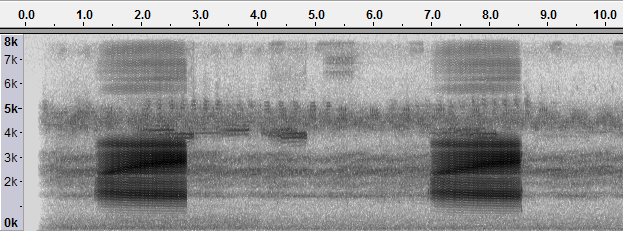
\includegraphics[width=45mm, height=30mm]{image/Ch1/graci_spec.png}     \end{minipage}    & 25.8  \\ \hline
\textit{Litoria latopalmata} &      \begin{minipage}{.3\textwidth} 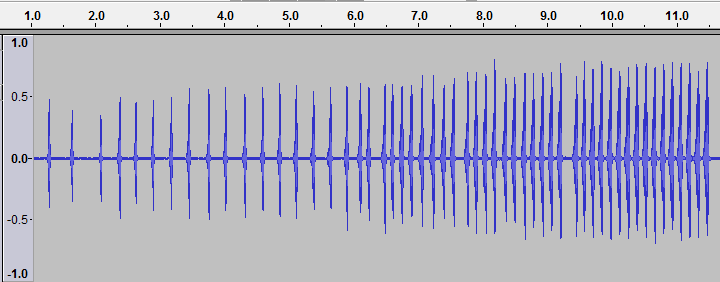
\includegraphics[width=45mm, height=30mm]{image/Ch1/latop_wav.png}  \end{minipage}  &    \begin{minipage}{.3\textwidth} 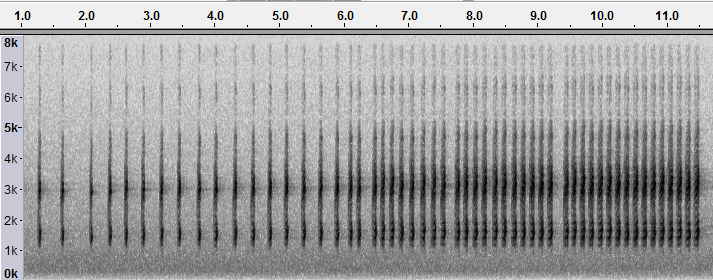
\includegraphics[width=45mm, height=30mm]{image/Ch1/latop_spec.png}    \end{minipage}     & 35.85 \\ \hline
\textit{Litoria rubella}     &   \begin{minipage}{.3\textwidth} 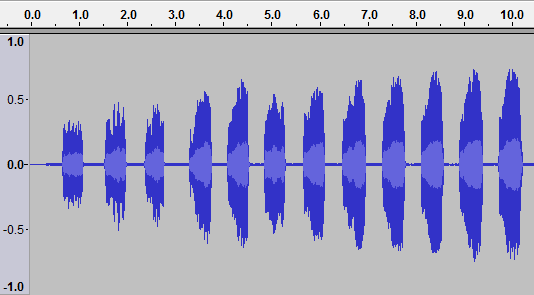
\includegraphics[width=45mm, height=30mm]{image/Ch1/rubella_wav.png}   \end{minipage}    &       \begin{minipage}{.3\textwidth} 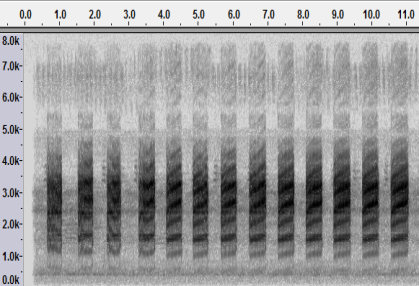
\includegraphics[width=45mm, height=30mm]{image/Ch1/rubella_spec.png}   \end{minipage}   & 36.2  \\ \hline\hline
\end{tabular}
\end{table}




\appendix[Waveform, spectrogram and SNR of eight frog species from JCU recordings]{Waveform, spectrogram and SNR of six frog species from JCU recordings} 

\begin{table}[htb!]
\centering
\caption[Waveform, spectrogram, and SNR of JCU recordings]{Waveform, spectrogram, and SNR of eight frog species (recordings from JCU)}
\label{tab:JCU_para}
\resizebox{\textwidth}{!}{
\begin{tabular}{llll}
\hline\hline
                            & Waveform & Spectrogram & SNR (dB) \\ \hline
\textit{Bufo marinus}                &   \begin{minipage}{.3\textwidth} 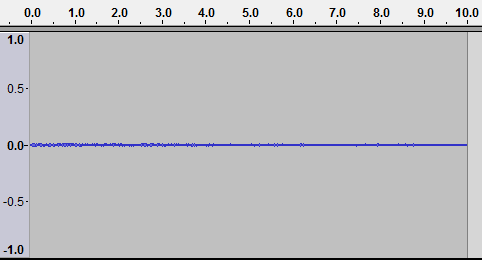
\includegraphics[width=45mm, height=30mm]{image/Ch1/toad_jcu_wav.png}  \end{minipage}       &      \begin{minipage}{.3\textwidth} 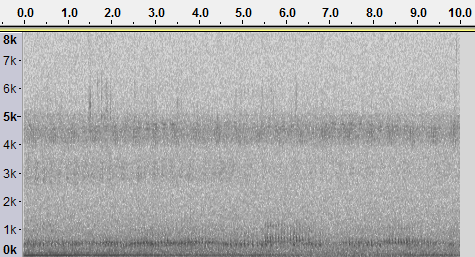
\includegraphics[width=45mm, height=30mm]{image/Ch1/toad_jcu_spec.png}  \end{minipage}       & 1.86     \\ \hline
\textit{Cyclorana novaehollandiae}   &  \begin{minipage}{.3\textwidth} 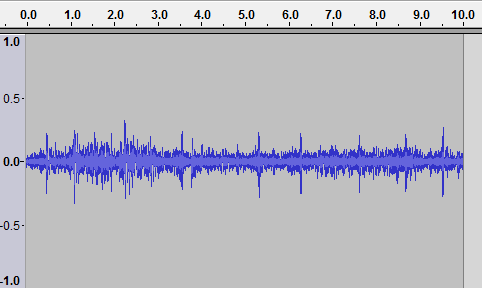
\includegraphics[width=45mm, height=30mm]{image/Ch1/cyc_jcu_wav.png}  \end{minipage}        & \begin{minipage}{.3\textwidth} 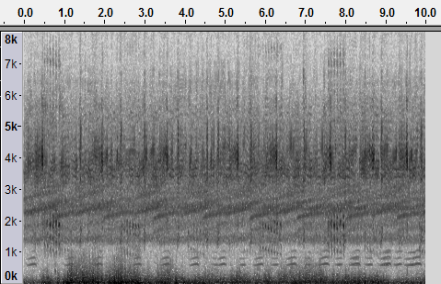
\includegraphics[width=45mm, height=30mm]{image/Ch1/cyc_jcu_spec.png}  \end{minipage}            & -0.13    \\ \hline
\textit{Limnodynastes terraereginae} &  \begin{minipage}{.3\textwidth} 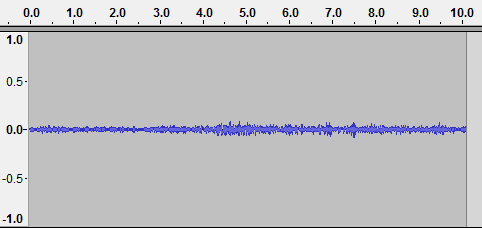
\includegraphics[width=45mm, height=30mm]{image/Ch1/ter_jcu_wav.png}  \end{minipage}        &   \begin{minipage}{.3\textwidth} 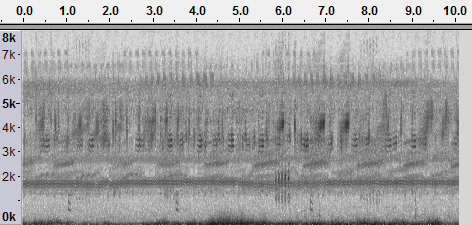
\includegraphics[width=45mm, height=30mm]{image/Ch1/ter_jcu_spec.png}  \end{minipage}          & -2.88    \\ \hline
\textit{Litoria fallax}              &   \begin{minipage}{.3\textwidth} 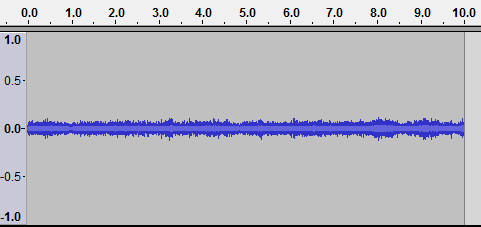
\includegraphics[width=45mm, height=30mm]{image/Ch1/fallax_jcu_wav.png}  \end{minipage}       &    \begin{minipage}{.3\textwidth} 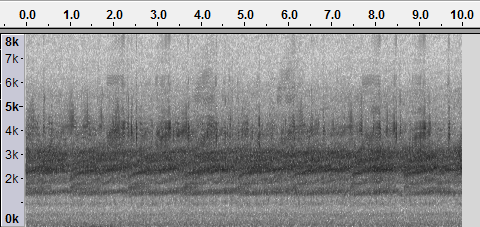
\includegraphics[width=45mm, height=30mm]{image/Ch1/fallax_jcu_spec.png}  \end{minipage}         & 1.52     \\ \hline
\end{tabular}
}
\end{table}


\begin{table}[htb!]
\centering
\resizebox{\textwidth}{!}{
\begin{tabular}{llll}
\hline
\textit{Litoria nasuta}              &   \begin{minipage}{.3\textwidth} 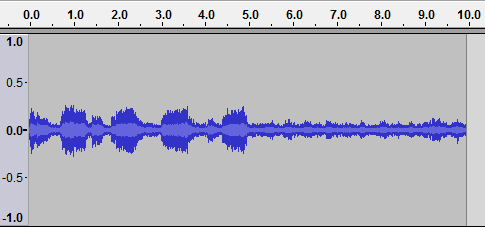
\includegraphics[width=45mm, height=30mm]{image/Ch1/nasuta_jcu_wav.png}  \end{minipage}       &  \begin{minipage}{.3\textwidth} 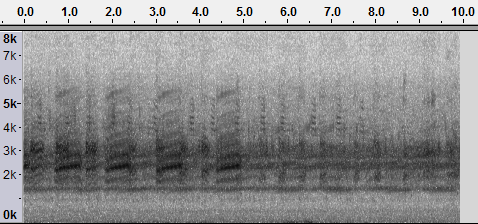
\includegraphics[width=45mm, height=30mm]{image/Ch1/nasuta_jcu_spec.png}  \end{minipage}           & 2.14     \\ \hline
\textit{Litoria rothii}              &   \begin{minipage}{.3\textwidth} 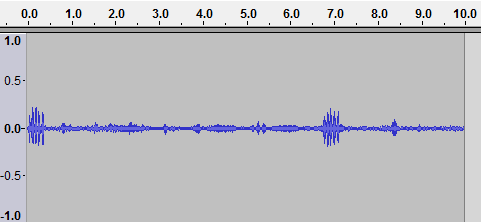
\includegraphics[width=45mm, height=30mm]{image/Ch1/rothii_jcu_wav.png}  \end{minipage}       &    \begin{minipage}{.3\textwidth} 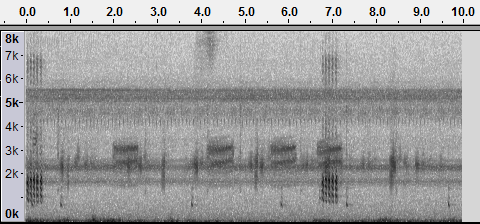
\includegraphics[width=45mm, height=30mm]{image/Ch1/rothii_jcu_spec.png}  \end{minipage}         & 10.24    \\ \hline
\textit{Litoria rubella}            &    \begin{minipage}{.3\textwidth} 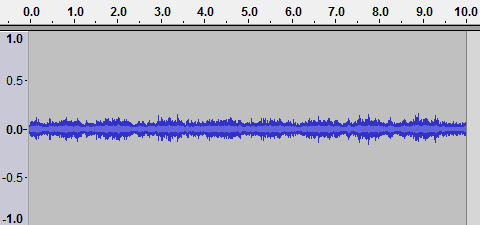
\includegraphics[width=45mm, height=30mm]{image/Ch1/rubella_jcu_wav.png}  \end{minipage}      &   \begin{minipage}{.3\textwidth} 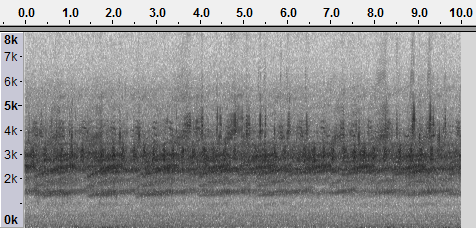
\includegraphics[width=45mm, height=30mm]{image/Ch1/rubella_jcu_spec.png}  \end{minipage}          & 1.08     \\ \hline
\textit{Uperolela mimula}            &   \begin{minipage}{.3\textwidth} 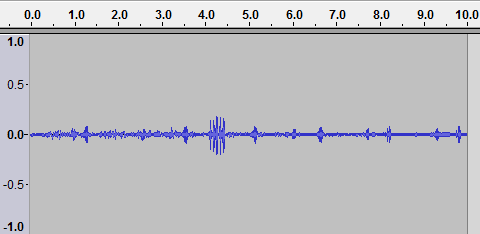
\includegraphics[width=45mm, height=30mm]{image/Ch1/mimula_jcu_wav.png}  \end{minipage}       &  \begin{minipage}{.3\textwidth} 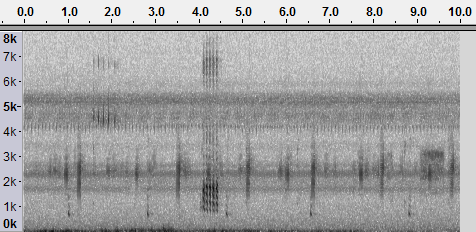
\includegraphics[width=45mm, height=30mm]{image/Ch1/mimula_jcu_spec.png}  \end{minipage}           & 10.28    \\ \hline\hline
\end{tabular}
}
\end{table}


\appendix[Power spectral density (PSD) estimate of signal and noise (JCU recordings)]{Power spectral density (PSD) estimate of signal and noise (JCU recordings)} 


\begin{table}[htb!]
\centering
\caption[PSD of JCU recordings]{Power spectral density (PSD) estimate of signal and noise (JCU recordings); for some frog species, the PSD difference between the signal and background noise is marked with the red rectangle, which indicates the frequency location of specific frog species; for others, the PSD of signal and noise is very similar, which means that some sources have similar frequency information with frog species}
\label{tab:psd}
\resizebox{\textwidth}{!}{
\begin{tabular}{lll}
\hline\hline
  \backslashbox{Frog \\ species}{Parameters}                           & Welch PSD (Signal) & Welch PSD estimate (Noise) \\ \hline
\textit{Bufo marinus}                &  \begin{minipage}{.3\textwidth} 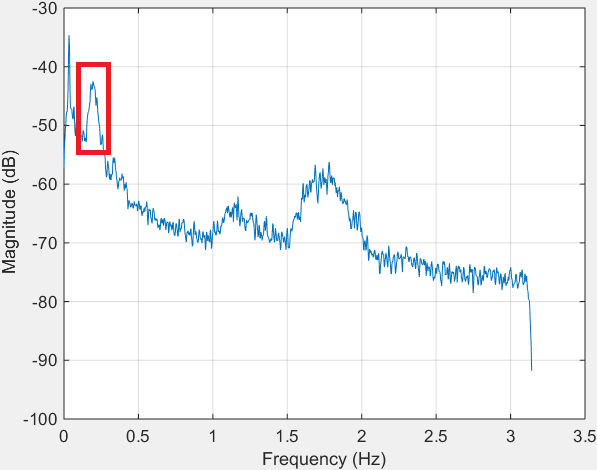
\includegraphics[width=45mm, height=35mm]{image/Ch1/1_signal.png}  \end{minipage}       &      \begin{minipage}{.3\textwidth} 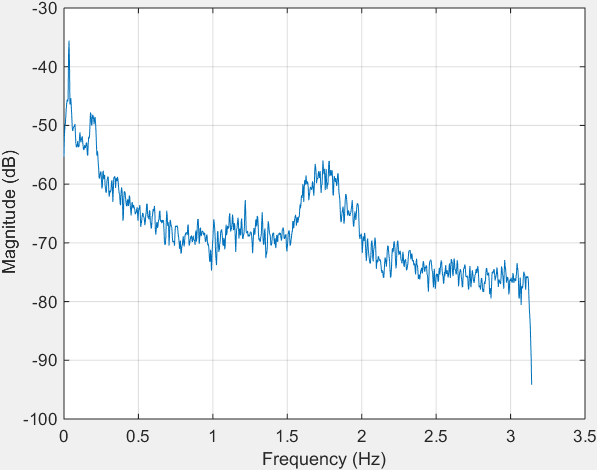
\includegraphics[width=45mm, height=35mm]{image/Ch1/1_noise.png}  \end{minipage}          \\ \hline
\begin{tabular}[c]{@{}l@{}} \textit{Cyclorana} \\ \textit{novaehollandiae}  \end{tabular}    & \begin{minipage}{.3\textwidth} 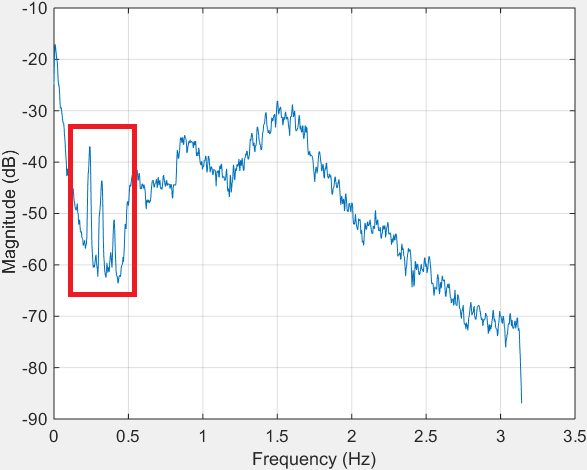
\includegraphics[width=45mm, height=35mm]{image/Ch1/2_signal.png}  \end{minipage}                              &                                              \begin{minipage}{.3\textwidth} 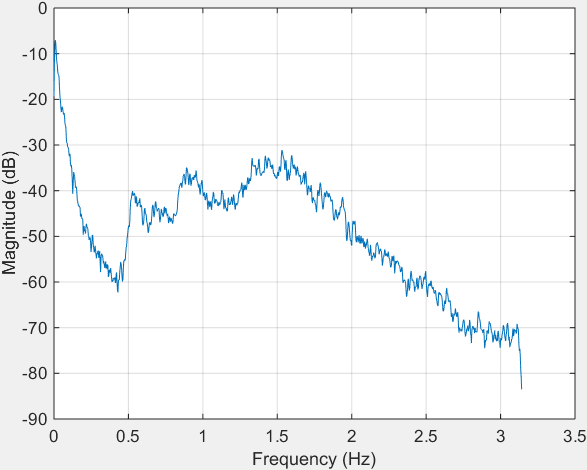
\includegraphics[width=45mm, height=35mm]{image/Ch1/2_noise.png}  \end{minipage}   \\ \hline

\end{tabular}
}
\end{table}


\begin{table}[htb!]
\centering
\resizebox{\textwidth}{!}{
\begin{tabular}{lll}
\hline
 \begin{tabular}[c]{@{}l@{}} \textit{Limnodynastes} \\ \textit{terraereginae}  \end{tabular}  &  \begin{minipage}{.3\textwidth} 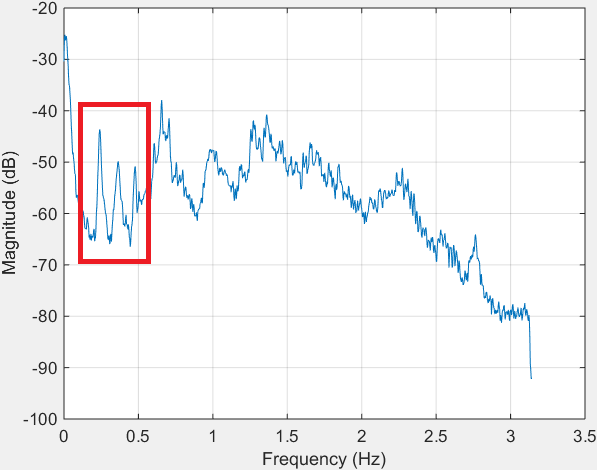
\includegraphics[width=45mm, height=35mm]{image/Ch1/3_signal.png}  \end{minipage}                              &                                             \begin{minipage}{.3\textwidth} 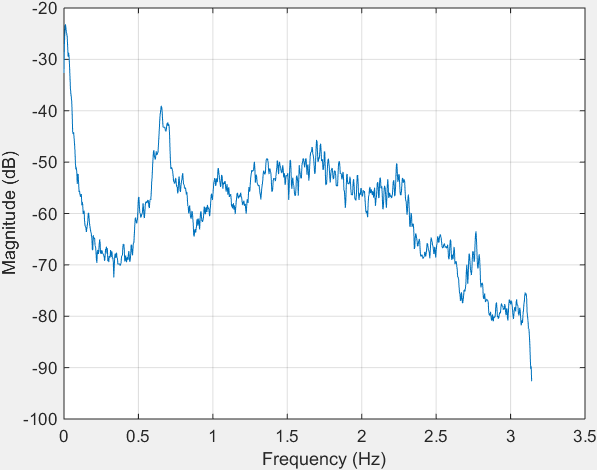
\includegraphics[width=45mm, height=35mm]{image/Ch1/3_noise.png}  \end{minipage}   \\ \hline
\textit{Litoria fallax}              & \begin{minipage}{.3\textwidth} 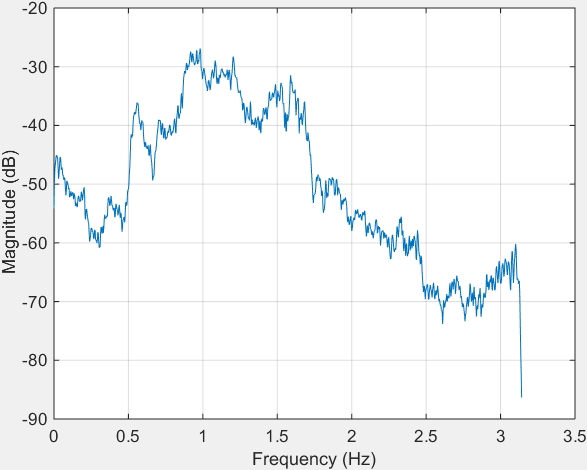
\includegraphics[width=45mm, height=35mm]{image/Ch1/4_signal.png}  \end{minipage}                             &                                               \begin{minipage}{.3\textwidth} 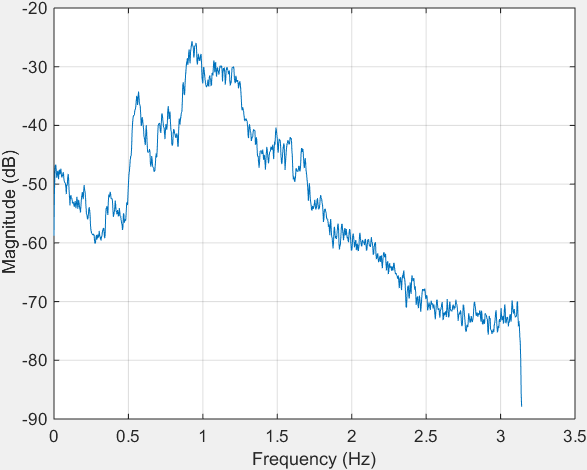
\includegraphics[width=45mm, height=35mm]{image/Ch1/4_noise.png}  \end{minipage} \\ \hline
\textit{Litoria nasuta}              &   \begin{minipage}{.3\textwidth} 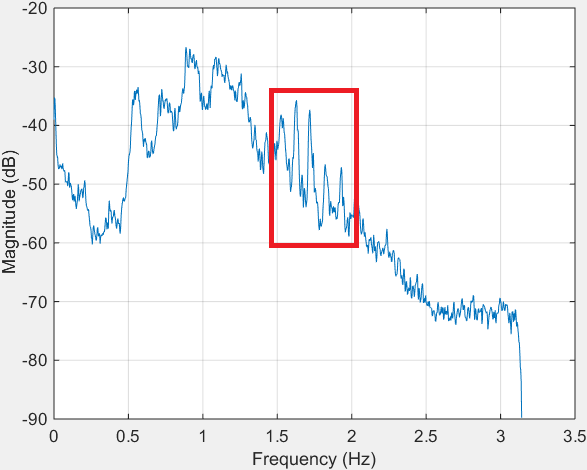
\includegraphics[width=45mm, height=35mm]{image/Ch1/5_signal.png}  \end{minipage}                           &                                               \begin{minipage}{.3\textwidth} 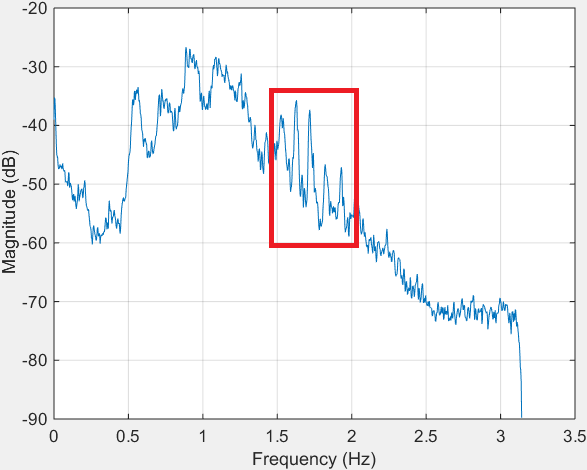
\includegraphics[width=45mm, height=35mm]{image/Ch1/5_signal.png}  \end{minipage} \\ 
\hline
\textit{Litoria rothii}             &  \begin{minipage}{.3\textwidth} 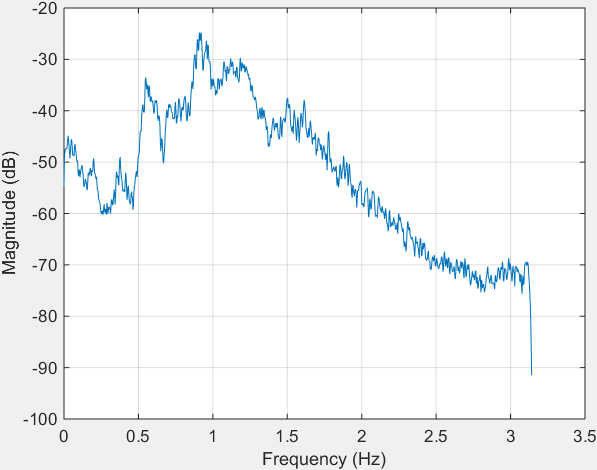
\includegraphics[width=45mm, height=35mm]{image/Ch1/6_signal.png}  \end{minipage}                         &    \begin{minipage}{.3\textwidth} 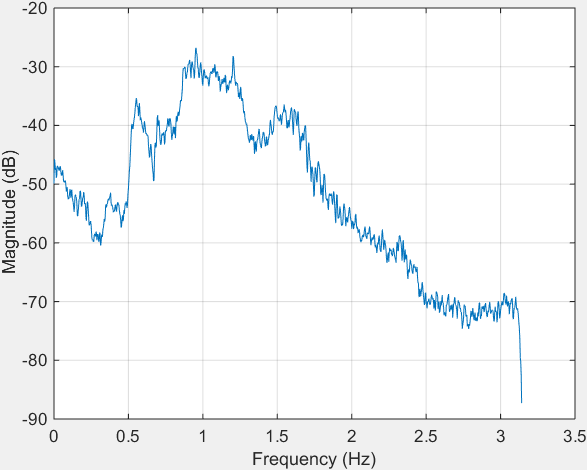
\includegraphics[width=45mm, height=35mm]{image/Ch1/6_noise.png}  \end{minipage}                                           \\ \hline
\textit{Litoria rubella}             &    \begin{minipage}{.3\textwidth} 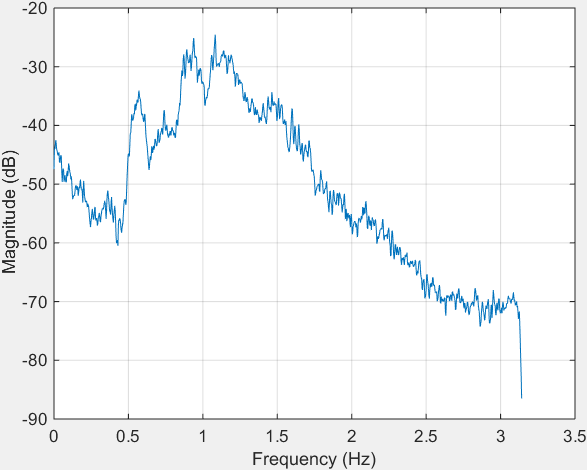
\includegraphics[width=45mm, height=35mm]{image/Ch1/7_signal.png}  \end{minipage}                               &                                               \begin{minipage}{.3\textwidth} 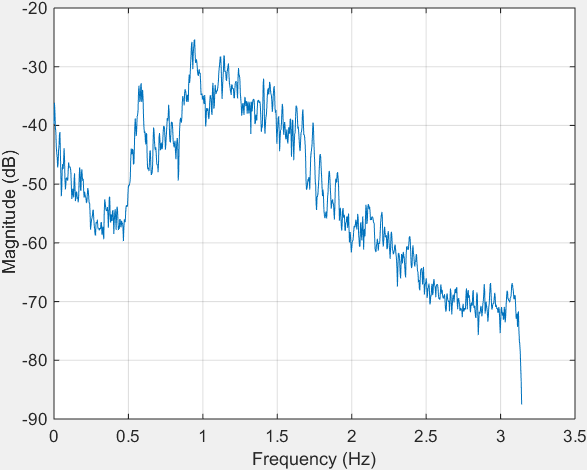
\includegraphics[width=45mm, height=35mm]{image/Ch1/7_noise.png}  \end{minipage} \\ \hline
\textit{Uperolela mimula}            &   \begin{minipage}{.3\textwidth} 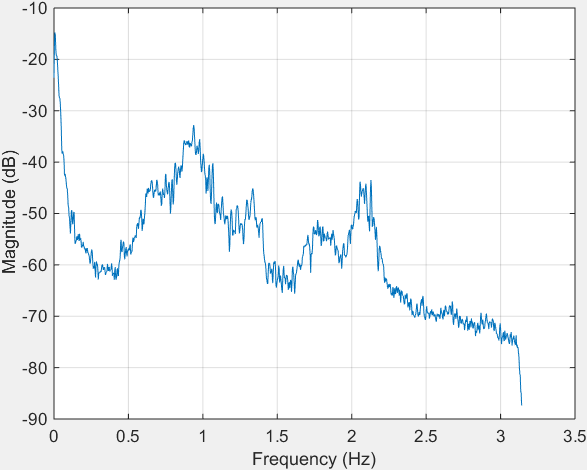
\includegraphics[width=45mm, height=35mm]{image/Ch1/8_signal.png}  \end{minipage}                              &                                             \begin{minipage}{.3\textwidth} 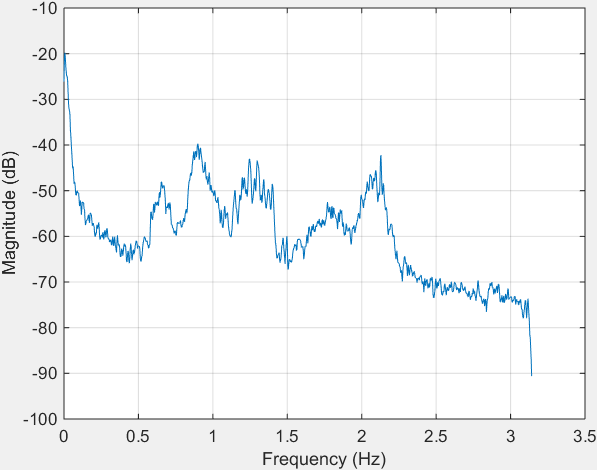
\includegraphics[width=45mm, height=35mm]{image/Ch1/8_noise.png}  \end{minipage} \\ \hline\hline
\end{tabular}
}
\end{table}














\appendix[Frog species studied in this study]{Frog species studied in this study} 
\label{app:A}







